\chapter{Continuité et dérivabilité}
\begin{abstract}
Dans ce chapitre, nous nous intéresserons aux notions de continuité et de dérivabilité, les espaces nécessaires ayant été définis précédemment, ainsi que les notions d'application...

Dans la mesure où les problèmes que nous souhaitons aborder, i.e. ceux issus de la physique, sont généralement décrits par des équations différentielles ou des équations aux dérivées partielles, on comprend bien que la notion de dérivation est centrale.

Mais n'oublions pas que ces notions de continuité et de différentiabilité n'ont pas toujours été définies de manière précise au cours de l'histoire et ont donné lieu à de bien terribles affrontements entre nos glorieux anciens.
\end{abstract}



\medskip
\section{Continuité et classe~$C^0$}\index{continuité!$C^0$}

\medskip
\begin{histoire}%
Dans le manuscrit de 1673 \emph{la Méthode inverse des tangentes ou à propos des fonctions}, Leibniz\index[aut]{Leibniz (Gottfried Wilhelm), 1646-1716, Allemand} dit:  «J'appelle fonctions toutes les portions des lignes droites qu'on fit en menant des droites indéfinies qui répondent au point fixe et aux points de la courbe; comme sont abscisse, ordonnée, corde, tangente, perpendiculaire, sous-tangente, sous-perpendiculaire... et une infinité d'autres d'une construction plus composée, qu'on ne peut figurer.»
Finalement, au terme d'une correspondance nourrie entre Leibniz\index[aut]{Leibniz (Gottfried Wilhelm), 1646-1716, Allemand} et Jean Bernoulli,\index[aut]{Bernoulli (Jean), 1667-1748, Suisse} celui-ci donne en 1718 la définition suivante: «On appelle fonction d'une grandeur variable une quantité composée, de quelque manière que ce soit, de cette grandeur variable et des constantes.».
Il propose la notation~$\phi x$.

La continuité est en quelque sorte contenue, sous-jacente à ces définitions car les fonctions considérées sont «physiques» et ne présentent au plus qu'un nombre fini de discontinuités.

\sbox{\MaBoiteAvecPhotos}{\setlength{\tabcolsep}{0pt}\scriptsize%
\begin{tabular}{ccc}%
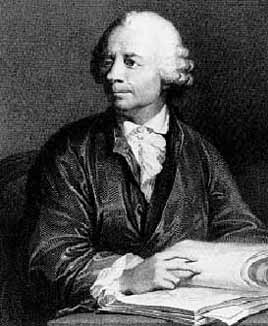
\includegraphics[height=\the\HauteurDesPhotos]{Euler3}&%
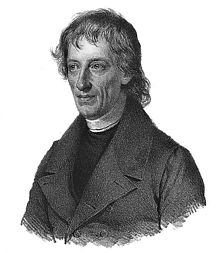
\includegraphics[height=\the\HauteurDesPhotos]{Bolzano}&%
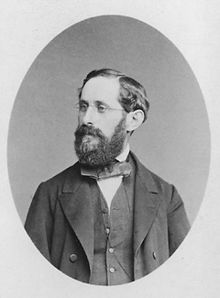
\includegraphics[height=\the\HauteurDesPhotos]{Heine}\\%
Euler &Bolzano&Heine%
\end{tabular}}
\medskip
\ImageADroite{%
Dans son \emph{Introductio in analysin infinitorum} de 1748, Euler\index[aut]{Euler (Leonhard Paul), 1707-1783, Suisse} définit une fonction d'une quantité variable comme «une expression analytique composée d'une manière quelconque de cette quantité variable et de nombres ou de quantités constantes». Le mot «analytique» n'est pas davantage précisé.
En fait, pour Euler, une fonction\index[aut]{Euler (Leonhard Paul), 1707-1783, Suisse} est une combinaison quelconque d'opérations prises dans le stock des opérations et des modes de calcul connus de son temps, et applicables aux nombres: opérations classiques de l'algèbre, exponentielle, logarithme, passage d'un arc à ses lignes trigonométriques..., certaines de ces opérations pouvant être itérées un nombre illimité de fois...\\ \indent
Dans ce même ouvrage, Euler\index[aut]{Euler (Leonhard Paul), 1707-1783, Suisse} dit qu'une fonction est continue si elle est définie par une seule expression anlytique (finie ou infinie) et mixte ou discontinue si elle possède plusieurs expression analytiques suivant ses intervalles de définition.\\ \indent
La définition actuelle est celle due à Bernard Bolzano\index[aut]{Bolzano (Bernard Placidus Johann Nepomuk), 1781-1848, Allemand} dans sa théorie des fonctions en 1816: «La fonction~$f(x)$ varie suivant la loi de continuité pour la valeur~$x$ si la différence~$| f(x + w) -f(x) |$ peut-être rendue plus petite que toute valeur donnée.»
Il existe une notion de continuité uniforme qui est plus forte que la simple continuité et fixée par Heinrich Eduard Heine\index[aut]{Heine (Eduard), 1821-1881, Allemand} en 1872.}
\end{histoire}
%\colorblack


\medskip
La continuité est une propriété topologique (donc indépendante de la métrique).
\medskipvm
\begin{definition}[Continuité d'une fonction en un point (version topologique)]
Soit~$f$ une application d'un espace topologique~$E$ dans un espace topologique $F$.
On dit que \textcolorblue{$f$ est continue en un point}~$a$ de~$E$ si, quelque soit le voisinage~$W$ de~$f(a)$ dans~$F$, il existe un voisinage~$V$ de~$a$ dans~$E$ tel que $\forall x\in V$, $f(x)\in W$, c'est-à-dire que l'image réciproque de tout voisinage de~$f(a)$ est un voisinage de~$a$.
\end{definition}
\medskipvm
\textcolorgris{Cette définition est donnée pour la culture, car nous n'avons pas rappelé la notion de voisinage dans ce document. Cela n'a pas d'importance dans ce contexte puisque nous travaillerons sur des cas moins généraux.}

\medskip
Évidemment, une application de~$E$ dans~$F$ est \textcolorblue{continue} si elle est continue en tout point de~$E$.
\medskipvm
Ramenons nous à des choses plus connues et plus en lien avec ce document.
Dans le cas des espaces métriques, la continuité se définit comme suit.

\begin{definition}[Continuité d'une fonction en un point (version métrique)]
Soient~$(E,d)$ et~$(E',d')$ deux espaces métriques, $f: E \to E'$ et~$a \in E$.
On dit que l'application~$f$ est continue en~$a$ si:
\begin{equation}
  \forall \varepsilon > 0, \quad \exists \eta > 0, \quad \forall x \in E, \quad \Bigl[d(x,a)<\eta \implies d'(f(x),f(a))<\varepsilon\Bigr]
\end{equation}
Ainsi~$f$ est continue en~$a$ si et seulement si la limite de~$f$ en~$a$ existe (elle vaut alors nécessairement~$f(a)$).
\end{definition}

\medskip
Considérons la fonction~$f$ définie sur~$\RR^2$ par:
\begin{equation}
  f(x,y)=\left\{\begin{aligned}&\frac{xy}{x^2+y^2}&&\text{ si } (x,y)\neq(0,0) \\
&0&&\text{ si } (x,y)=(0,0) \end{aligned}\right.
\end{equation}
Elle n'a pas de limite en~$(0,0)$.

\colorgris\small
En effet, $f(x,y)$ est continue partout sur~$\RR^2\backslash\{(0,0)\}$. Elle est continue sur l'axe des abscisses et des ordonnées où elle est~$\equiv0$. Elle est donc séparément continue à l'origine, et par suite dans tout le plan. Mais elle n'est pas continue par rapport à l'ensemble des variables à l'origine, car sur la droite~$y=mx$, elle prend la valeur~$m/(1+m^2)$ en dehors de l'origine; or~$\frac{m}{1+m^2}\ne0$ dès que~$m\ne0$, et par conséquent elle ne tend pas vers~$0$ lorsque~$(x,y)$ tend vers l'origine. Une telle fonction est dite partiellement continue.\colorblack
\normalsize

\medskip
\textcolorred{Pour une fonction réelle, on peut définir une fonction continue comme une fonction dont on peut tracer le graphe sans lever le crayon}. Si l'on exclut certains fonctions très particulières (comme les fractales), alors l'idée générale de la continuité est bien traduite par cette phrase (la fonction ne présente pas de «saut»).

\medskip
%Définie de cette manière simple, une fonction~$f: I\subset\RR \to \RR$ sera dite \textcolorblue{continue
%au point~$a\in I$} si:
\begin{definition}[Continuité d'une fonction réelle en un point]
Une fonction~$f: I\subset\RR \to \RR$ sera dite \textcolorblue{continue au point~$a\in I$} si:
\begin{equation}
  \forall \varepsilon > 0, \quad \exists \eta > 0, \quad \forall x \in I, \quad \Bigl[|x - a| <\eta \implies |f(x) - f(a)|<\varepsilon\Bigr].
\end{equation}
\end{definition}

\medskip
\textcolorblue{La classe des fonctions continues} est notée~$C^0$.
Elle inclut par exemple les fonctions continues par morceaux ainsi que les constantes (dont la fonction nulle).

\medskip
Attention à ne pas confondre la classe des fonctions continues~$C^0$ avec $C_0$ l'ensemble des fonctions continues qui s'annulent à l'infini (sous-espace de l'espace des fonctions continues).

\medskip
\section{Continuité de Hölder et Lipschitz}\index{continuité!Hölder}\index{continuité!Lipschitz}\index[aut]{Hoelder@Hölder (Otto Ludwig), 1859-1937, Allemand}\index[aut]{Lipschitz (Rudolph Otto Sigismund), 1832-1903, Allemand}

\colorgreen\textbf{Remarque:}
Dans le cas des espaces métriques, nous avons vu qu'il était possible de redéfinir la continuité à l'aide des~$\varepsilon$ plutôt que par les voisinages.\vskip15pt

\sbox{\MaBoiteAvecPhotos}{\setlength{\tabcolsep}{0pt}\scriptsize%
\begin{tabular}{cc}%
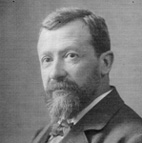
\includegraphics[height=\the\HauteurDesPhotos]{Holder}&%
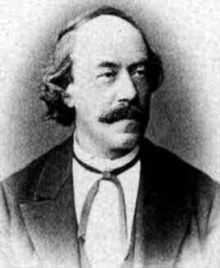
\includegraphics[height=\the\HauteurDesPhotos]{Lipschitz}\\%
Hölder &Lipschitz%
\end{tabular}}
\bigskip\ImageADroite{\colorgreen
Avec Hölder\index[aut]{Hoelder@Hölder (Otto Ludwig), 1859-1937, Allemand} et Lipschitz,\index[aut]{Lipschitz (Rudolph Otto Sigismund), 1832-1903, Allemand} la notion de «continuité uniforme» nous est proposée.
La distinction entre continuité et continuité uniforme est la même que celle entre la convergence simple et la convergence uniforme dans le cas des séries (pour le lecteur qui s'en souviendrait).
En effet, cette continuité uniforme ne regarde pas comment (quel~$\varepsilon$) la fonction est continue en chaque point, mais comment elle est continue dans sa globalité, i.e. lorsque ce fameux~$\varepsilon$ n'est plus lié à la position sur la courbe, mais est fixé pour la fonction entière.}
\colorblack
\medskipvm
La \textcolorblue{continuité höldérienne} ou \textcolorblue{condition de Hölder} est une condition suffisante (mais non nécessaire) pour qu'une application définie entre deux espaces \textcolorred{métriques} soit continue.

La définition s'applique en particulier pour les fonctions d'une variable réelle.

\medskip
\begin{definition}[Fonction~$a$-höldérienne]
Si~$(E, d)$ et~$(F, d')$ sont deux espaces métriques, une fonction~$f: E \rightarrow F$ est dite $a$-höldérienne s'il existe une constante~$C > 0$ telle que:
\begin{equation}
  \forall (x, y) \in \mathrm{e}^2,\quad d'\left(f(x), f(y)\right) \le C\,d\left(x,y\right)^a
\end{equation}
\end{definition}
La continuité höldérienne d'une fonction dépend donc d'un paramètre réel strictement positif~$a \in \intof{0}{1}$, et prend en compte toutes les variations de la valeur de la fonction sur son ensemble de définition.
\parvm
Si~$0 < a \le 1$ est fixé, l'ensemble des fonctions réelles~$a$-höldériennes est un espace vectoriel, conventionnellement noté~$\mathcal{C}^{0, a}(E,\RR)$.

\medskip
\begin{theoreme}
Toute application~$f$ qui est~$a$-höldérienne est continue. Mieux, elle est \textcolorblue{uniformément continue}, dans le sens suivant:
\begin{equation}
\text{Si } \varepsilon>0\text{, alors pour } \eta = \left( \varepsilon / C \right)^{1 / a},\quad d\left( x, y \right) < \eta \ \Rightarrow\ d\left( f(x), f(y) \right) < \varepsilon
\end{equation}
Le réel~$\eta$ dépend de~$\varepsilon$ mais est indépendant de la variable~$x$ parcourant l'espace de définition de l'application.
\end{theoreme}
\medskipvm
\begin{definition}[Fonction lipschitzienne]
Lorsque~$a = 1$, l'application est dit \textcolorblue{lipschitzienne}.
Une application lipschitzienne est plus «régulière» qu'une fonction simplement continue.
\end{definition}
Toute fonction lipschitzienne (en tant que fonction höldérienne) est uniformément continue.
\parvm
Toute fonction réelle lipschitzienne est (absolument continue donc à variation bornée donc) dérivable presque partout pour la mesure de Lebesgue et sa dérivée est essentiellement bornée.

\medskip
\section{Dérivée}\index{dérivée!classique}

Le nombre dérivé en un point d'une fonction à variable et valeurs réelles est le coefficient directeur de la tangente au graphe de cette fonction en ce point, ou aussi le coefficient directeur de l'approximation affine de cette fonction en ce point: ce nombre n'est donc défini que si cette tangente, ou cette approximation, existe.
La dérivée d'une fonction $f$ est une fonction qui, à tout nombre pour lequel $f$ admet un nombre dérivé, associe ce nombre dérivé.
%\medskipvm
\begin{definition}[Dérivée d'une fonction]
Soit~$f$ une application d'un ouvert~$\Omega$ du corps~$\KK$ (resp. un intervalle de~$\RR$) dans un espace affine normé~$F$ (resp.~$\RR$), alors on peut donner un sens, pour~$a\in\Omega$, à la quantité:
\begin{equation}\label{Eq-derivee}
f'(a)=\lim_{\substack{h\ne0,h\to0\\a+h\in\Omega}} \dfrac{f(a+h)-f(a)}h \in F
\end{equation}
que l'on appelle le vecteur dérivé ou simplement la \textcolorblue{dérivée} de $f$ en~$a$.
\end{definition}
\medskipvm
\begin{histoire}%
Au \textsc{xvii}\fup{e} siècle, la compréhension mais surtout la modélisation (i.e. la mise en équations) de phénomènes physiques et techniques conduit à la création au siècle suivant de l'analyse en tant que branche des mathématiques abordant les notions de dérivation, intégration et équations différentielles.

\sbox{\MaBoiteAvecPhotos}{\setlength{\tabcolsep}{0pt}\scriptsize%
\begin{tabular}{cc}%
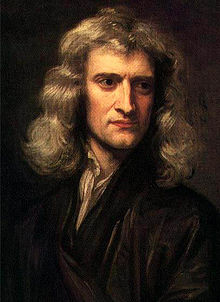
\includegraphics[height=\the\HauteurDesPhotos]{Newton}&%
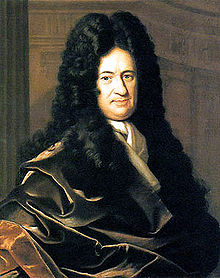
\includegraphics[height=\the\HauteurDesPhotos]{Leibniz}\\%
Newton &Leibniz%
\end{tabular}}
\medskip
\ImageADroite{%
Les échanges, les conceptions et la compréhension des infinitésimaux ont animé le monde scientifique pendant bien longtemps, la discussion était tout autant philosophique que mathématique, ce qui est somme toute assez normal compte tenu du sujet...
Les fondateurs incontestés de l'analyse sont Newton\index[aut]{Newton (Isaac, Sir -), 1643-1727, Anglais} et Leibniz.\index[aut]{Leibniz (Gottfried Wilhelm), 1646-1716, Allemand}
La portée de ces travaux est considérable car ils vont permettre non seulement la compréhension des courbes (puis le calcul des aires), mais aussi celle du mouvement des corps.
C'est véritablement une révolution où l'on passe d'une science de la statique à une
science de la dynamique.}

Un débat houleux sur la paternité du calcul différentiel entre mathématiciens britanniques et allemands fit rage, mais Newton et Leibniz s'en tinrent à l'écart.
Toutefois, cette polémique entre les deux camps ne sera pas sans effet.
Celle-ci fera que les anglais resteront à l'écart du développement général des mathématiques au \textsc{xviii}\fup{e} siècle, la tradition newtonienne dominante ayant abouti à une certaine stagnation scientifique. Au début du \textsc{xix}\fup{e} siècle, avec la diffusion des notations symboliques leibniziennes du calcul infinitésimal, un petit groupe de mathématicien de Cambridge se mettront à réfléchir sur le rôle et l'importance de la symbolique.

\medskip
L'opinion générale est aujourd'hui que Leibniz s'est presque certainement inspiré de certaines des idées de Newton (dont les travaux sont antérieurs, mais non publiés au moment où Leibniz publie), mais que sa contribution reste suffisamment importante pour que le mérite de l'invention du calcul différentiel soit accordé aux deux hommes.

L'approche de Newton est proche de la physique: il parle en termes de mouvement physique et ses notations ne sont employées que très rarement en dehors de la sphère des physiciens.

L'approche de Leibniz en revanche est plus géométrique et conduit à une présentation plus naturelle, encore utilisée aujourd'hui, et qui va rapidement être adoptée en Europe. C'est lui également qui introduit la notation~$dy/dx$ encore utilisée.

\sbox{\MaBoiteAvecPhotos}{\setlength{\tabcolsep}{0pt}\scriptsize%
\begin{tabular}{cc}%
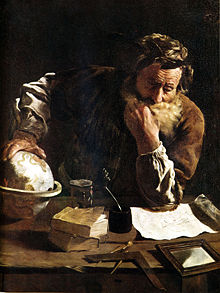
\includegraphics[height=\the\HauteurDesPhotos]{Archimede}&%
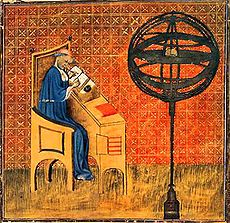
\includegraphics[height=\the\HauteurDesPhotos]{Oresme}\\%
Archimède&Oresme%
\end{tabular}}
\medskip
\ImageAGauche{%
Avant Newton et Leibniz, Descartes\index[aut]{Descartes (René), 1596-1650, Français} s'était intéressé au problème des tangentes à une courbe et Fermat\index[aut]{Fermat (Pierre, de -), ?-1665, Français} avait introduit une notion assez de la dérivée lors d'une recherche d'extremum.
En remontant encore plus dans l'Histoire, on peut dire que la méthode d'exhaustion, telle qu'elle a été développée et utilisée par Archimède\index[aut]{Archimède de Syracuse, -287-- -212, Grec} (i.e. avec toute la rigueur nécessaire, en usant du procédé d'encadrement évitant le recourt aux~$\varepsilon$) est réellement la première utilisation des infinitésimaux.
Malgré, ou peut-être à cause de, la grande originalité de ses travaux, Archimède\index[aut]{Archimède de Syracuse, -287-- -212, Grec} n'a été que peu suivi dans le monde grec et n'a pas eu de disciple direct.\\
\indent
Les savants arabes commenceront d'ailleurs dès le \textsc{ix}\fup{e} siècle à s'intéresser aux procédés infinitésimaux mis en œuvre par le génial Alexandrin.}

\medskip
Notons également que le plus grand progrès théorique réalisé au Moyen-Âge est l'étude quantitative de la variabilité par Nicole Oresme\index[aut]{Oresme (Nicole), 1325-1382, Allemand}.
Éveillé par la diffusion des méthodes infinitésimales des Anciens, et d'Archimède\index[aut]{Archimède de Syracuse, -287-- -212, Grec} en particulier, nourri par les spéculations scolastiques sur l'infini, le goût des mathématiciens pour les considérations infinitésimales se développe peu à peu. Ils s'appliquent d'abord à imiter le modèle archimédien, puis s'émancipent et essaient de trouver des substituts pour la méthode d'exhaustion, jugée trop lourde.

\medskip
En 1748, Euler\index[aut]{Euler (Leonhard Paul), 1707-1783, Suisse} définit les deux nouvelles opérations que sont la différentiation et l'intégration dans \emph{Introductio in analysin infinitorum}, puis dans \emph{Calculi differentialis} (1755) et \emph{Institutiones calculi integralis} (1770) essaie de mettre au point les règles d'utilisation des infiniment petits et développe des méthodes d'intégration et de résolution d'équations différentielles.

\medskip
Enfin, dans la seconde moitié du \textsc{xix}\fup{e} siècle, on s'intéressera aux propriétés des fonctions dérivées, et de nombreux contre-exemples défiant l'intuition seront introduits, qui conduiront à bien cerner cette délicate notion.
\end{histoire}
\colorblack

\medskip
La dérivabilité est elle-aussi une notion topologique et non métrique (même si on sait l'écrire en termes métrique comme ci-dessus), elle ne dépend donc pas de la norme choisie (du moment que celle-ci est compatible avec la topologie choisie...).


\medskip
\section{Fonctions de classe~$C^k$}\index{continuité!$C^k$}

Il est évident que si la dérivée (telle que définie au dessus) existe partout dans $\Omega$, alors on peut à nouveau considérer sa dérivée... et ainsi de suite.

On définit donc les \textcolorblue{classes~$C^1$, $C^2$, ...~$C^k$, ...~$C^\infty$} de fonctions 1 fois, 2 fois, ..., $k$ fois continûment dérivables ou même indéfiniment dérivables.
\medskipvm
Pour~$k=0$, on retombe sur la définition de l'ensemble des fonctions continues.
\medskipvm
Pour être très clair, \textcolorred{une fonction est de classe~$C^k$ signifie que toutes ses dérivées jusqu'à l'ordre~$k$ sont continues dans~$\Omega$}.
\medskipvm
Toutes les fonctions polynomiales sont~$C^\infty$, car à partir d'un certain rang leur dérivée est identiquement nulle.

\medskip
\section{Différentielle}\label{Sec-Differentielle}%\index{dérivée!partielle}

Il s'agit de généraliser la formule~\ref{Eq-derivee} à des applications de~$\RR^n$ dans~$\RR^p$. La variable étant maintenant un vecteur de~$\RR^n $, il n'est plus question de diviser par~$h$... il faut donc modifier la définition pour supprimer le dénominateur. Et cela est très facile: il suffit d'approcher l'accroissement de la fonction par une application linéaire.
\begin{definition}[Différentielle]
Soient $E$ et $F$ deux espaces normés sur le corps $\KK=\RR$ ou $\CC$, et $U$ un ouvert de $E$. Une application $f: U\rightarrow F$ est dite \textcolorblue{différentiable au point $a\in U$} s'il existe une application linéaire $L\in\mathcal{L}(E,F)$ telle que:
\begin{equation}
f(a+h)-f(a)=L(h)+R(h)
\end{equation}
où le reste $R(h)$ est un $o(\|h\|)$ lorsque $h$ tend vers $0$ dans $E$.

\medskip
Si elle existe, l'application $L$ est unique et on l'appelle la \textcolorblue{différentielle} de $f$ en $a$.
On la note $L=Df(a)$, ou $f'(a)$ ou $df(a)$ ou $D_af$ ou $df_a$, selon les auteurs et les circonstances.
\end{definition}
Cela signifie qu'au voisinage de~$a$, l'application~$f$ se comporte à peu près comme l'application affine $x\mapsto f(a)+Df(a)(x-a)$, pour laquelle on pourra utiliser les outils de l'algèbre linéaire. Géométriquement, on retrouve l'idée qu'une courbe est, au voisinage d'un point, à peu près confondues avec sa tangente\footnote{tangente, du latin «tangerer»: toucher} (droite tangente, plan tangent...). C'est pourquoi l'application linéaire~$Df(a)$ est également appelée application linéaire tangente à~$f$ en~$a$.

\medskip
Évidemment, dans le cas où~$E=\RR$ et~$F=\RR$, tout ce qui a été dit coïncide avec ce que nous avions vu avec la dérivée classique.

\medskip
\section{Dérivées partielles}\index{dérivée!partielle}

Nous nous intéressons maintenant au cas où une fonction dépend de plusieurs variables, i.e. au cas d'une fonction numérique d'une variable vectorielle. Avec les notation du paragraphe précédent, cela correspond au cas où~$E=\RR^n$ et~$F=\RR$.

\medskip
\textcolorblue{La dérivée partielle d'une fonction de plusieurs variables est la dérivée par rapport à l'une de ses variables, les autres étant gardées constantes.}
\medskipvm
La dérivée partielle de la fonction~$f$ par rapport à la variable~$x$ est notée $\frac{ \partial f}{ \partial x}$ ou~$\partial_x f$ ou encore~$f'_x$.
\medskipvm
De la même manière, on peut noter des dérivés secondes,...~$k$-ièmes par rapport à différentes variables.
Par exemple~$\frac{ \partial^2 f}{ \partial x^2} = f_{xx}' = \partial_{xx} f = \partial^2_x f$, mais également~$\frac{ \partial^2 f}{\partial x\,\partial y} = f_{yx}' = \partial_{yx} f$, ou $\frac{ \partial^2 f}{\partial y\,\partial x} = f_{xy}' = \partial_{xy} f~$, mais également $\frac{ \partial^{i+j+k} f}{ \partial x^i\, \partial y^j\, \partial z^k} = f_{kz jy ix}' = \partial_{kz jy ix} f~$.

\medskip
\begin{definition}[Dérivée partielle d'ordre 1 en un point]
%La définition se fait de manière analogue au cas de la dérivée «classique».

Soient~$\Omega$ un ouvert de~$\RR^n$ et~$f$ une fonction de~$n$ variables:
\begin{equation}
f: \begin{array}{ccc}
\Omega &\to& \RR\\
 \mathbf{x} = (x_1,\dots,x_n) &\mapsto& f(\mathbf{x}) = f(x_1,\dots,x_n)
\end{array}\end{equation}
On définit la \textcolorblue{dérivée partielle d'ordre 1 de~$f$ au point~$\mathbf{a} = (a_1,\dots,a_n) \in \Omega$
par rapport à la~$i$-ème variable~$x_i$} par:
\begin{equation}
  \frac{ \partial f}{\partial x_i}(\mathbf{a}) = \lim_{h \to 0}{ f(a_1, \dots , a_{i-1}, a_i+h, a_{i+1}, \dots ,a_n) - f(a_1, \dots ,a_n) \over h}
\end{equation}
\end{definition}

\begin{remarque}
Pour en revenir au cadre général qu'est celui de la différentielle, on parle ici des dérivées partielles pour désigner les dérivées dans la direction des vecteurs de base, ou plus exactement des dérivées selon les vecteurs de base.

\medskip
Nous utiliserons, comme tout le monde, la notation $\frac{ \partial f}{ \partial x_i}$, bien qu'elle présente quelques défauts: tout d'abord elle est typographiquement lourde, ensuite elle a les apparences trompeuses d'un quotient, et enfin la mention  de la variable $x_i$ peut être source de confusions dans les calculs de dérivées de fonctions composées. On devrait donc toujours préférer la notation $\partial_if$ ou $f'_i$.

\medskip
La formulation générale de la différentielle donnée au paragraphe~\ref{Sec-Differentielle} permet de retrouver tous les cas:
\begin{itemize}
   \item le cas «classique» d'une fonction d'une variable réelle à valeur réelle correspond au cas $E=\RR$ et~$F=\RR$;
   \item le cas d'une fonction numérique d'une fonction vectorielle correspond au cas $E=\RR^n$ et~$F=\RR$ et vient d'être présenté. Dans ce cas, la différentielle~$Df(\mathbf{a})$ est la forme linéaire sur~$\RR^n$ de composantes~$\LL{\partial_1f(\mathbf{a}), ..., \partial_nf(\mathbf{a})}$ dans la base canonique.
   
   Si~$\RR^n$ est muni d'un produit scalaire, alors il existe un unique vecteur, appelé \textcolorblue{gradient} de~$f$ en~$\mathbf{a}$ et noté~$\gradb f(\mathbf{a})\in\RR^n$ tel que: $Df(\mathbf{a})h=\gradb f(\mathbf{a}).h$. Pour une définition plus opérationnelle du gradient, on se réfèrera au paragraphe~\ref{Sec-nabla}. Celui-ci a pour composantes les dérivées partielles par rapport à la base considérée;
   \item le cas d'une fonction vectorielle d'une variable réelle correspond au cas $E=\RR$ et~$F=\RR^p$. Il est à nouveau possible de diviser par~$h$. La différentiabilité\footnote{On ne confondra pas «différencier» et «différentier»} de~$f$ équivaut alors à la dérivabilité de ses composantes~$f_i$.

   \item le cas d'une fonction vectorielle d'une variable vectorielle correspond au cas le plus général $E=\RR^n$ et~$F=\RR^p$. La différentielle est l'application linéaire définie dans les bases canoniques de~$\RR^n$ et~$\RR^p$ par la matrice \textcolorblue{jacobienne}. La ligne~$i$ de la matrice jacobienne correspond à la différentielle de la composante~$f_i$ de~$f$. La colonne~$j$ de la matrice jacobienne correspond à la dérivée de~$f$ dans la direction du~$j$\fup{e} vecteur de la base. Nous y reviendrons de manière plus pragmatique au paragraphe~\ref{Sec-Jacob}.
\end{itemize}
\end{remarque}

\medskip
\textcolorred{Attention:}
Même si toutes les dérivées partielles~$\frac{ \partial f}{\partial x_1}(\mathbf{a}),\, \dots,\, \frac{ \partial f}{\partial x_n}(\mathbf{a})$ existent en un point~$\mathbf{a}$, la fonction peut ne pas être continue en ce point.
Si l'on considère à nouveau la fonction~$f$ définie sur~$\RR^2$ par:
\begin{equation}
  f(x,y)=\left\{\begin{aligned}&\frac{xy}{x^2+y^2}&&\text{ si } (x,y)\neq(0,0)\\
&0&&\text{ si } (x,y)=(0,0)\end{aligned}\right.
\end{equation}
on voit qu'elle vérifie~$\frac{\partial f}{\partial x} (0,0)= \frac{\partial f}{\partial y} (0,0)=0$ mais elle n'a pas de limite en~$(0,0)$ comme nous l'avons vu avant.


\medskip
Si \textcolorred{toutes} les dérivées partielles (d'ordre 1) existent et sont \textcolorred{continues} dans un voisinage de~$\mathbf{a}$, alors~$f$ est différentiable dans ce voisinage et la différentielle est continue. Dans ce cas, on dit que~$f$ est une fonction de \textcolorblue{classe~$C^1$} sur ce voisinage de~$\mathbf{a}$.

Si \textcolorred{toutes} les dérivées partielles secondes de~$f$ existent et sont \textcolorred{continues} sur l'ouvert~$\Omega$, on dit que~$f$ est une fonction de \textcolorblue{classe~$C^2(\Omega)$}.
L'ordre de dérivation peut alors être changé sans que cela modifie le résultat.
C'est le \textcolorblue{théorème de Schwarz}\index[aut]{Schwarz (Hermann Amandus), 1843-1921, Allemand} \textcolorgris{(Il s'agit de Hermann Amandus Schwarz (sans «t»), pas de Laurent Schwartz)}.
\begin{theoreme}[Théorème de Schwarz]
Si~$f\in C^2(\Omega)$, alors:
\begin{equation}\colorred
  \frac{\partial^2f}{\partial x_i\, \partial x_j} = \frac{\partial^2f} {\partial x_j\, \partial x_i}
\end{equation}
\end{theoreme}
%\footnotetext{
%\begin{tabular}{c}
%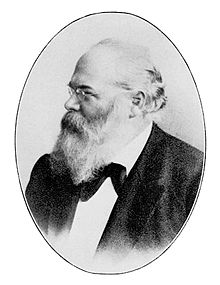
\includegraphics[height=32mm]{Schwarz}\\
%Hermann Amandus Schwarz\\
%1843-1921\\
%\end{tabular}
%}

\begin{definition}[Différentielle totale]
On appelle \textcolorblue{différentielle totale} de~$f$ l'expression:
\begin{equation}
  \dd f=\frac{\partial f}{\partial x_1}\,\dd x_1+\cdots+\frac{\partial f}{\partial x_n}\,\dd x_n
=  \dsum_i \frac{\partial f}{\partial x_i}\,\dd x_i
\end{equation}
\end{definition}

\medskip
\section{Retour sur les classes~$C^k$ pour une fonction de plusieurs variables}

Ce paragraphe met l'accent sur le cas multi-dimensionnel des classes~$C^k$ (ce qui est le cas avant, mais peut-être moins visiblement). Nous en profitons également pour introduire des notations et notions dont nous nous servirons plus loin.

\medskip
\begin{definition}[Fonctions~$k$ fois différentiables]
Si~$\Omega$ est un ouvert de~$\RR^n$, on définit l'ensemble des fonctions~$k$ fois différentiables dans~$\Omega$, à valeurs dans~$\RR$ dont toutes les dérivées jusqu'à l'ordre~$k$ sont continues dans $\Omega$ par:
\begin{equation}
C^k(\Omega) = \left\{f\in C^{k-1}(\Omega), \dfrac{\partial f}{\partial x_i}\in C^{k-1}(\Omega),
i=1, ..., n\right\}, k\ge 1
\end{equation}
\end{definition}

\medskip
\begin{definition}[Multi-indice]
On appelle \textcolorblue{multi-indice}~$\alpha$ un~$n$-uplet d'entiers $\alpha=(\alpha_1, ..., \alpha_n)$, $\alpha_j\in\NN$.
Sa \textcolorblue{longueur} est~$|\alpha|=\alpha_1+ ... + \alpha_n$, et on note \textcolorblue{$\partial^\alpha$} la quantité (l'opération)
\begin{equation}
   \partial^\alpha=\left(\dfrac{\partial}{\partial x_1}\right)^{\alpha_1}...\left(\dfrac{\partial}{\partial x_n}\right)^{\alpha_n}\end{equation}
\end{definition}

\medskip\colorgris
$C^k(\Omega)$ est l'espace vectoriel des fonctions~$f: \Omega \to \RR$ telles que $\forall \alpha$, $|\alpha|\le k$, $x\mapsto \partial^\alpha f(x)$ existe et appartient à~$C^0(\Omega)$.

Pour~$f$ et~$g$ dans~$C^k(\Omega)$, on définit:
\begin{equation}
d(f,g)=\dsum_{i=1}^\infty \dfrac1{2^i}\dfrac{\dsum_{|\alpha|\le k} \sup_{K_i}|\partial^\alpha f(x)-g(x)|}{%
1+\dsum_{|\alpha|\le k} \sup_{K_i}|\partial^\alpha f(x)-g(x)|}
\end{equation}
qui est une distance sur~$C^k(\Omega)$ qui en fait un espace complet. L'espace~$C^\infty(\Omega)$ peut se définir par:
\begin{equation} C^\infty(\Omega)=\bigcup\limits_{k\in\NN}C^k(\Omega)\end{equation}
qui est également complet pour la même distance.
%\textcolorblue{Cette définition permet de clairement voir les inclusions successives des espaces~$C^k$.}

\bigskip\colorblack
On définit également~$C^k_b(\Omega)$ comme le sous-espace vectoriel des éléments de~$C^k(\RR^n)$ dont \textcolorblue{toutes les dérivées jusqu'à l'ordre~$k$ sont bornées} sur~$\Omega$.

On définit alors:
\begin{equation}
\|f\|_{C^k_b(\Omega)}=\dsum_{|\alpha|\le k} \sup_{\Omega} |\partial^\alpha f(x)|
\end{equation}
qui est une norme sur~$C^k_b(\Omega)$ et en fait un espace de Banach (i.e. normé complet pour cette norme).

\medskip
\begin{definition}\label{Def-Cc}
On définit, pour~$k\in\NN\cup\{\infty\}$, l'ensemble \textcolorblue{$C_c^k(\Omega)$} par:
$f\in C_c^k(\Omega)$ si~$f\in C^k(\Omega)$ et si~$f$ est de support compact inclus dans~$\Omega$.
\end{definition}
Pour tout ouvert~$\Omega$ de~$\RR^n$, et pour tout~$k\in\NN\cup\{\infty\}$:
\begin{itemize}
  \item~$C_c^k(\Omega)$ est dense dans~$C^k(\Omega)$;
  \item~$C_c^\infty(\Omega)$ est dense dans~$C^k(\Omega)$.
\end{itemize}

\medskip
\section{Nabla et comparses}\label{Sec-nabla}

\subsection{Champs de vecteurs et de scalaires}

\begin{definition}[Champ de vecteurs]
Soit~$E$ un espace vectoriel euclidien\index[aut]{Euclide, -325-- -265, Grec} de dimension~$n$ et~$\Omega$ un ouvert de E.
Un \textcolorblue{champ de vecteurs} sur~$\Omega$ est une application~$F$ de~$\Omega$ dans~$E$, définie par ses~$n$ fonctions composantes:
\begin{equation}
  F: \VV*{x_1\\\vdots\\x_n} \longmapsto \VV*{F_1(x_1,\dots,x_n)\\ \vdots\\ F_n(x_1,\dots,x_n)}
\end{equation}
C'est donc une fonction qui à un vecteur fait correspondre un vecteur.
\end{definition}

\begin{definition}[Champ de scalaires]
Un \textcolorblue{champ de scalaires} sur~$\Omega$ est une application~$f$ de~$\Omega$ dans~$\RR$ ou~$\CC$, i.e. une fonction qui à un vecteur fait correspondre un scalaire.
\end{definition}
La dérivée d'un champ scalaire est un champ vectoriel appelé \textcolorblue{gradient} (voir plus bas).

\medskip
\colorblue Nabla, noté~$\nabla$, est un pseudo-vecteur \colorblack servant à noter un opérateur différentiel:
\begin{equation}
\nabla = \VV*{{\dfrac\partial{\partial x}}\\ \dfrac\partial{\partial y}\\ \dfrac\partial{\partial z}}_{\text{cartésiennes}}
= \VV*{\dfrac\partial{\partial \rho}\\ \dfrac1\rho \dfrac\partial{\partial \varphi}\\ \dfrac\partial{\partial z}}_{\text{polaires}}
= \VV*{\dfrac\partial{\partial r}\\ \dfrac1r \dfrac\partial{\partial \theta}\\\dfrac1{r\sin\theta} \dfrac\partial{\partial \varphi}}_{\text{sphériques}}
\end{equation}

\medskip
\subsection{Gradient, divergence, rotationnel, Laplacien et D'Alembertien}\index{gradient}\index{divergence}\index{rotationnel}\index{laplacien}\index{d'Alembertien}

Les quantités présentées ci-après apparaîtront constamment dans les problèmes physiques.%

\medskip
Soient~$\mathbf{A}~$ un champ de vecteur et~$f$ un champ scalaire, on définit:
\begin{itemize}
\item Le \textcolorblue{gradient}:
\begin{equation} \gradb f \equiv \nabla f \end{equation}

\item La \textcolorblue{divergence}:
\begin{equation} \dive \mathbf{A} \equiv \nabla\cdot\mathbf{A} \end{equation}

\item Le \textcolorblue{rotationnel}:
\begin{equation} \rotb \mathbf{A} \equiv \nabla \wedge \mathbf{A} \end{equation}

\item Le \textcolorblue{Laplacien} (scalaire et vectoriel):
\begin{align} &\Delta f = \nabla^2 f\\
&\Delta \mathbf{A} = \nabla^2 \mathbf{A} \end{align}

\item Le \textcolorblue{D'alembertien}: il s'agit plus d'une «contraction d'écriture».
En coordonnées cartésiennes, $\Box$ s'écrit:
\begin{equation}
  \Box = \frac{1}{c^2}\frac{\partial^2}{\partial t^2} - \left(\frac{\partial^2}{\partial x^2} + \frac{\partial^2}{\partial y^2} + \frac{\partial^2}{\partial z^2}\right)
  = \frac{1}{c^2}\frac{\partial^2}{\partial t^2} - \Delta
\end{equation}
\end{itemize}
où~$c$ est la vitesse de la propagation considérée (ou la vitesse de la lumière).

\medskip
En coordonnées cartésiennes, il vient explicitement:
\begin{itemize}
  \item gradient:~$ \gradb f=
	\VV*{{\partial f \over \partial x}\\ {\partial f \over \partial y}\\ {\partial f \over \partial z}}$
  \item divergence:~$ \dive \mathbf{A} =
	{\partial A_x \over \partial x} + {\partial A_y \over \partial y} + {\partial A_z \over \partial z}$
  \item rotationnel:~$ \rotb \mathbf{A} =
	\VV*{{\partial A_z \over \partial y} - {\partial A_y \over \partial z} \\
	{\partial A_x \over \partial z} - {\partial A_z \over \partial x} \\
	{\partial A_y \over \partial x} - {\partial A_x \over \partial y}}$
  \item Laplacien scalaire:~$\Delta f ={\partial^2 f \over \partial x^2} + {\partial^2 f \over \partial y^2} + {\partial^2 f \over \partial z^2}$
  \item Laplacien vectoriel:~$\Delta \mathbf{A} =
	\VV*{\Delta A_x \\ \Delta A_y \\ \Delta A_z}$
\end{itemize}

\medskip
De plus:
\begin{align}
&\dive \gradb f = \nabla \cdot (\nabla f) = \nabla^2 f = \Delta f\\
&\rotb\gradb f = \nabla \wedge ( \nabla f)
\colorred = \boldsymbol 0\\
&\dive\rotb \mathbf{A} = \nabla \cdot ( \nabla \wedge \mathbf{A} ) \colorred = 0\\
&\rotb\rotb\mathbf{A} = \nabla \wedge (\nabla \wedge \mathbf{A} ) =\nabla ( \nabla \cdot \mathbf{A} ) - \nabla^2 \mathbf{A} = \gradb\dive \mathbf{A} - \Delta \mathbf{A} \\
&\Delta f g = f \Delta g + 2 \nabla f \cdot \nabla g + g \Delta f
\end{align}

\medskip
\subsection{Normale et dérivée normale}\index{dérivée!normale}\index{normale}

\begin{definition}[Normale]
On appelle \textcolorblue{normale} au domaine~$\Omega$ un champ de vecteurs $n(x)$ défini sur le bord~$\Gamma=\partial\Omega$ de~$\Omega$ et tel qu'en tout point $x\in\Gamma$ où le bord est régulier, $n(x)$ soit orthogonal au bord et de norme~$1$.
\end{definition}

\medskip
On appelle \textcolorblue{normale extérieure} une normale qui pointe vers l'extérieur du domaine en tout point.

\medskip
\begin{definition}[Dérivée normale]
On appelle \textcolorblue{dérivée normale} d'une fonction régulière~$u$ sur~$\Gamma$, la fonction définie sur les points réguliers de~$\Gamma$ par:
\begin{equation}\dfrac{\partial u}{\partial n}(x)=\nabla u(x)\cdot n(x)\end{equation}
Il s'agit d'un produit scalaire car~$\nabla u$ est un vecteur, tout comme~$n(x)$.
\end{definition}

\medskip
\subsection{Potentiel d'un champ vectoriel}

Le \textcolorblue{potentiel d'un champ vectoriel} est une fonction scalaire ou vectorielle qui, sous certaines conditions relatives au domaine de définition et à la régularité, permet des représentations alternatives de champs aux propriétés particulières. Ainsi:
\begin{itemize}
  \item Un champ vectoriel irrotationnel (de rotationnel nul) peut être identifié au gradient d'un potentiel scalaire.
  \item Un champ vectoriel solénoïdal (de divergence nulle) peut être identifié au rotationnel d'un potentiel vecteur.
\end{itemize}
Dans les deux cas, on dit que le champ d'origine \textcolorblue{dérive d'un potentiel} (allusion entre une fonction et sa primitive).

\medskip
Ces potentiels permettent non seulement d'appréhender certains champs vectoriels sous un angle complémentaire (pour un traitement parfois plus aisé), mais ils légitiment des abstractions essentielles comme, par exemple en physique, l'énergie potentielle associée à un champ de forces conservatives.

\medskip
Un champ de vecteurs~$\mathbf{A}$ continu et irrotationnel dérive d'un potentiel scalaire~$U$:
\begin{equation}
 \mathbf{A} = -\gradb U
\end{equation}
Le même résultat se vérifie dans l'espace entier à condition que, vers l'infini, le champ décroisse «assez» rapidement.

Le potentiel scalaire n'est pas unique, il est défini à une constante près.

\medskip
Un champ de vecteurs~$\mathbf{A}$ régulier et de divergence nulle dérive d'un potentiel vectoriel
$\mathbf{B}~$:
\begin{equation}
  \mathbf{A} = -\rotb \mathbf{B}
\end{equation}
Le même résultat se vérifie dans l'espace entier à condition que, vers l'infini, le champ
décroisse «assez» rapidement.

Le potentiel vecteur n'est pas unique, il est défini à un «gradient» près (i.e. $ \mathbf{B} ' = \mathbf{B} + \gradb f$ convient également).

\medskip
\subsection{Signification «physique»}

Un \textcolorgreen{champ de scalaires}, c'est un «truc», une application, qui à un vecteur associe un scalaire. Typiquement, on peut penser à la \textcolorgreen{température}.
Une application~$T(x,y,z)$ qui à chaque point de l'espace de coordonnées~$(x,y,z)$ associe sa température~$T$ est un champ de scalaire.

Un \textcolorgreen{champ de vecteurs}, c'est un «truc», une application, qui à un vecteur associe un autre vecteur. Typiquement, on peut penser à la \textcolorgreen{vitesse}.
Une application~$\mathbf{V}(x,y,z)$ qui à chaque point de l'espace de coordonnées~$(x,y,z)$ associe son vecteur vitesse~$\mathbf{V}$ est un champ de vecteurs.

\medskip
Si~$f$ est une fonction de classe~$C^1$, alors le \textcolorgreen{gradient} de~$f$ au point~$\mathbf{a}$, quand il est non nul, s'interprète comme la direction selon laquelle~$f$ varie le plus vite, i.e. la ligne de plus grande pente.

La \textcolorgreen{divergence} d'un champ de vecteurs mesure comment son courant déforme un volume \textcolorgris{(on devrait dire comment son flot déforme une forme volume au sens de la géométrie différentielle)}.
{\small L'idée est un peu la suivante: imaginons un écoulement de fluide et intéressons-nous au courant en fonction de la profondeur. Lorsque l'on est un peu en dessous de la surface et loin du sol, on peut imaginer que le courant est à peu près constant, donc une section (ou un volume) de fluide perpendiculaire à l'écoulement se retrouve, un instant plus tard, un peu plus loin, mais toujours perpendiculaire au sol, i.e. la section n'a pas varié. Si l'on est proche du fond, on peut penser que le courant est plus faible très près du sol, par exemple à cause du frottement. Si l'on considère à nouveau une section de fluide perpendiculaire au sol, alors un instant plus tard, elle n'est plus perpendiculaire au sol: près du sol, les particules ont effectué un petit déplacement, celles plus éloignées ont beaucoup plus avancé. La section n'a ni la même forme, ni la même longueur qu'à l'instant précédent. La divergence mesure justement ce type d'écart.}
\textcolorgreen{D'une manière plus générale, la divergence traduit la conservation (si elle est nulle) ou non d'une grandeur physique en un point: cela mesure donc, en chaque point si une grandeur (par exemple le volume comme avant) est conservative ou non.}


Le \textcolorgreen{rotationnel} exprime la tendance qu'ont les lignes de champ d'un champ vectoriel à tourner autour d'un point: sa circulation locale sur un petit lacet entourant ce point est non nulle quand son rotationnel ne l'est pas (nous n'avons pas défini la notion de lacet, nous compterons sur l'imagination du lecteur). \textcolorgris{On rappelle que les lignes de champ sont les lignes qui, en première approche, représente le chemin que l'on suivrait en partant d'un point.
Ce sont en fait les lignes orthogonales aux équipotentielles, ou surfaces de niveau, du champ.}

\medskip
Concernant le \textcolorgreen{Laplacien scalaire}, la quantité~$\Delta f$ est une mesure de la différence entre la valeur de~$f$ en un point quelconque~$P$ et la valeur moyenne~$\overline{f}$ au voisinage du point~$P$.

Le \textcolorgreen{Laplacien scalaire} d'une fonction peut aussi être interprété comme la courbure moyenne locale de la fonction, que l'on visualise aisément pour une fonction à une seule variable~$f(x)$.
La dérivée seconde (ou courbure)~$f''$ représente la déviation locale de la moyenne par rapport à la valeur au point considéré.

\bigskip
Les notions de rotationnel, gradient, Laplacien... interagissent. Par exemple en \textcolorgreen{mécanique des fluides}, le rotationnel de la vitesse décrit une rotation de la particule fluide.
Si l'écoulement est irrotationnel (son rotationnel est nul en tout point), alors le vecteur vitesse est le gradient du potentiel (on dit alors que les vitesses dérivent d'un potentiel).
Si le fluide peut être considéré comme incompressible, la divergence de ce vecteur s'annule.
Le laplacien du potentiel est donc nul: il s'agit d'un potentiel harmonique qui satisfait l'équation de Laplace.

\medskip
\section{Quelques théorèmes sur les intégrales}

Les relations ci-après permettent de passer d'intégrales sur un domaine à des intégrales sur le bord de ce domaine.


\medskip
\begin{theoreme}[Théorème du gradient]\index{gradient}\index{théorème!du gradient}
Ce théorème met en relation l'intégrale de volume du gradient d'un champ scalaire et l'intégrale de surface de ce même champ:
 \begin{equation}
  \int_\Omega \nabla f = \int_\Gamma f \vect{n}(x)
\end{equation}
où~$\Gamma$ est le bord du domaine~$\Omega$ et~$f$ un champ scalaire (i.e. une fonction régulière).
\end{theoreme}

\medskip
\begin{theoreme}[Théorème du rotationnel]\index{rotationnel}\index{théorème!du rotationnel}
Ce théorème met en relation l'intégrale de volume du rotationnel d'un champ vectoriel et l'intégrale de surface du même champ:
\begin{equation}
\int_\Omega \rotb \mathbf{A} =
-\int_\Gamma \mathbf{A} \wedge \vect{n}(x)
\end{equation}
où~$\Gamma$ est la frontière de~$\Omega$, $\wedge$ est le produit vectoriel et~$n(x)$ est la normale dirigé vers l'extérieur.
\end{theoreme}

\medskip\colorgris
Une autre identité remarquable met en relation l'intégrale de surface du rotationnel d'un champ vectoriel et l'intégrale curviligne (ou circulation) du même champ sur la frontière.
Elle découle du théorème de Green qui, pour une surface~$S$ (généralement non fermée) de frontière~$C$, implique:
\begin{equation}
\iint_S \rotb \mathbf{A} \cdot \dd\mathbf{s} = \oint_C \mathbf{A} \cdot \dd\mathbf{l}
\end{equation}
Si~$S$ est fermée, $C$ est vide (ou réduit à un point) et le membre de droite est nul.

\medskip
L'orientation de la surface et celle de la courbe frontière sont liées puisque le changement d'une orientation modifie le signe de l'intégrale correspondante.
En fait, la relation est satisfaite lorsque ces orientations sont telles que, sur un point frontière, le vecteur tangent à la surface~$\dd \vec s \wedge \dd \vec l$ est orienté en direction de la surface.
\colorblack


\medskip
\begin{theoreme}[Théorème de Green--Riemann]\index{théorème!de Green--Riemann}%
\index[aut]{Green (George), 1793-1841, Anglais}\index[aut]{Riemann (Georg Friedrich Bernhard), 1826-1866, Allemand}

Ce théorème donne la relation entre une intégrale curviligne autour d'une courbe simple fermée~$C$ et l'intégrale double sur la région du plan~$S$ délimitée par~$C$.

Soit~$C$, une courbe plane simple, positivement orientée et~$C^1$ par morceaux, $S$ le domaine compact lisse du plan délimité par~$C$ et  $P\dd x + Q\dd y$ une 1-forme différentielle sur~$\RR^2$. Si~$P$ et~$Q$ ont des dérivées partielles continues sur une région ouverte incluant~$S$, alors:
\begin{equation}
\int_C P\,\dd x + Q\,\dd y = \iint_S \left( \frac{\partial Q}{\partial x} - \frac{\partial P}{\partial y}\ \right) \dd x\dd y
\end{equation}
\end{theoreme}

\medskip\colorgris
Il existe une autre façon de noter ce théorème.
On se place sur un domaine compact lisse du plan~$\Omega$, de bord~$\partial\Omega$, en notant la forme différentielle~$\omega$.
Alors la dérivée extérieure de~$\omega$ s'écrit:
\begin{equation}
\dd \omega = \left( \frac{\partial Q}{\partial x} - \frac{\partial P}{\partial y} \right) \dd x \wedge \dd y
\end{equation}
On peut alors résumer le théorème de Green par la formule:
\begin{equation}
\oint_{\partial \Omega} \omega = \iint_{\Omega} \dd\omega
\end{equation}
(Le cercle sur l'intégrale précise que le bord décrit une courbe fermée).
\colorblack

\medskip
\begin{theoreme}[Théorème de Green--Ostrogradsky]\index[aut]{Green (George), 1793-1841, Anglais}%
\index[aut]{Ostrogradsky (Mikhaïl Vassilievitch), 1801-1862, Ukainien}\index{théorème!de Green-Ostrogradsky}\index{théorème!du flux-divergence}\index{divergence}
Soit~$\Omega$ un domaine de~$\RR^2$ ou~$\RR^3$ de frontière~$\Gamma$ et~$\mathbf{A}$ un champ de vecteurs:
\begin{equation}
  \int_\Omega \dive\ \mathbf{A} = \int_\Gamma \mathbf{A}\cdot n
\end{equation}
\end{theoreme}

\medskip
Ce théorème prend aussi le nom de théorème du flux-divergence ou plus simplement formule de la divergence. «Ostrogradsky» peut s'écrire avec un «y» ou un «i» à la fin. Du théorème de Green-Ostrogradsky, on peut déduire la formule de Green:\index[aut]{Green (George), 1793-1841, Anglais}

\begin{theoreme}[Formule de Green]
Soient~$\Omega$ un domaine de~$\RR^2$ ou~$\RR^3$ de frontière~$\Gamma$ et~$u$ et~$v$ deux fonctions régulières:
\begin{equation}
\int_\Omega (\Delta u)v = -\dint_\Omega \nabla u\cdot\nabla v + \dint_\Gamma \dfrac{\partial u}{\partial n}v
\end{equation}
\end{theoreme}

\medskip
On en déduit certaines formules utiles du calcul vectoriel.
Soit~$\Omega$ un domaine de~$\RR^2$ ou~$\RR^3$ de frontière~$\Gamma$, $\mathbf{A}$ et~$\mathbf{B}$ des champ de vecteurs, $f$ et~$g$ des fonctions régulières, et~$n(x)$ la normale extérieure au point considéré:
\begin{align}
  &\int_\Omega \left( \mathbf{A}\cdot \nabla f + f \left(\nabla \cdot \mathbf{A}\right)\right)=
  \int_\Gamma f \mathbf{A}\cdot n(x)\\
&\int_\Omega \left( \mathbf{B}\cdot\left(\nabla \wedge \mathbf{A}\right) - \mathbf{A}\cdot \left(\nabla
\wedge \mathbf{B}\right) \right)
= \int_\Gamma \left(\mathbf{A} \wedge \mathbf{B}\right)\cdot n(x)\\
&\int_\Omega \left( f \nabla^{2} g + \nabla f \cdot \nabla g \right)
= \int_\Gamma f \nabla g \cdot \vect{n}(x)
\end{align}
Ces formules sont exploitées pour obtenir des formulations faibles associées à des problèmes aux dérivées partielles. 
